
%----------------------------------------------------------------------------------------
%	PACKAGES AND OTHER DOCUMENT CONFIGURATIONS
%----------------------------------------------------------------------------------------

\documentclass{article}

\usepackage{fancyhdr} % Required for custom headers
\usepackage{lastpage} % Required to determine the last page for the footer
\usepackage{extramarks} % Required for headers and footers
\usepackage{graphicx} % Required to insert images
\usepackage{mathtools, bm}
\usepackage{amssymb, bm}
\usepackage{graphicx}
\usepackage{float}
\usepackage{multirow}
\usepackage[table]{xcolor}  
\usepackage{algorithm}
\usepackage[noend]{algpseudocode}

% Margins
\topmargin=-0.45in
\evensidemargin=0in
\oddsidemargin=0in
\textwidth=6.5in
\textheight=9.0in
\headsep=0.25in


\linespread{1.1} % Line spacing

% Set up the header and footer
\pagestyle{fancy}
\lhead{\hmwkAuthorName} % Top left header
\chead{\hmwkTitleComp} % Top center header
\rhead{\firstxmark} % Top right header
\lfoot{\lastxmark} % Bottom left footer
\cfoot{} % Bottom center footer
\rfoot{Page\ \thepage\ of\ \pageref{LastPage}} % Bottom right footer
\renewcommand\headrulewidth{0.4pt} % Size of the header rule
\renewcommand\footrulewidth{0.4pt} % Size of the footer rule

\setlength\parindent{0pt} % Removes all indentation from paragraphs

%----------------------------------------------------------------------------------------
%	DOCUMENT STRUCTURE COMMANDS
%	Skip this unless you know what you're doing
%----------------------------------------------------------------------------------------

% Header and footer for when a page split occurs within a problem environment


% Header and footer for when a page split occurs between problem environments
   
%----------------------------------------------------------------------------------------
%	NAME AND CLASS SECTION
%----------------------------------------------------------------------------------------
\newcommand{\logoepfl}{
  \begin{center}
    
\includegraphics[width=4cm]{img/epfl.jpg}
  \end{center}
  \vspace{0.3cm}
  \hrule
}


\newcommand{\hmwkTitle}{Decentralized Verifiable Computation on Distributed Ledger}
\newcommand{\hmwkTitleComp}{Decentralized Verifiable Computation on Distributed Ledger} % Assignment title
\newcommand{\hmwkDueDate}{Summer 2018} % Due date
\newcommand{\hmwkClass}{IN, LCA1} % Course/class
\newcommand{\hmwkClassTime}{} % Class/lecture time
\newcommand{\hmwkClassInstructor}{D.Froelicher, J.Troncoso-Pastoriza} % Teacher/lecturer
\newcommand{\hmwkAuthorName}{Max Premi} % Your name

%----------------------------------------------------------------------------------------
%	TITLE PAGE
%----------------------------------------------------------------------------------------
\title{
\logoepfl
\vspace{2in}
\textmd{\textbf{\hmwkClass:\ \hmwkTitle}}\\
\normalsize\vspace{0.1in}\small{Due\ on\ \hmwkDueDate}\\
\vspace{0.1in}\large{\textit{\hmwkClassInstructor\ \hmwkClassTime}}
\author{\textbf{\hmwkAuthorName}}
\vspace{3in}
}

%----------------------------------------------------------------------------------------

\begin{document}

\maketitle

\newpage
\section*{Abstract}
\addcontentsline{toc}{section}{Abstract}
Data sharing systems are becoming more popular these past years, and are used in several domains, such as economics [REF], software validation [REF], and even medical field [REF]. They eliminate singles point of failures, enforces transparency, and provides an efficient way to ensure security, authentication, and privacy.
The latter is required to respect privacy laws but introduces overhead such as encryption, verification of computation ( correctness), and tracking of error (robustness).\\
UnLynx is such a system that uses Elliptic curve ElGamal encryption, zero-knowledge proof, and noise addition, as well as several other protocols to maintains all properties stated above. However, it only supports a small subset of operation (sum, count, average), and it has a strong threat model.\\
This project is a part of a design of a new decentralized system Lemal, supporting a large set of operation (mean, variance, logistic regression,...), while keeping all properties in an efficient way, in addition of universal verifiability of computations and results.
In this project, we introduce a way to make all the proofs public and verifiable by anyone, through distributed ledger.
The goal of this project is to:
\begin{description}
\item[$\bullet$] First, propose a theoretical system implementation of the Skipchain, to create a Collective Authority of Verifying nodes that guarantees correctness and robustness of computation.
\item[$\bullet$] Then, implement protocols that handle the Skipchain operations, based on the previous implementation done by DeDis.
\item[$\bullet$] Implement the interface between the Collective authority doing the computation and the Collective authority of verifying nodes.
\item[$\bullet$] Finally, measure the performance of this system.
\end{description}

\newpage

\tableofcontents

\newpage

\section{Introduction}
Blockchain [REF] technology has emerged in 2008, with the Bitcoin, that use distributed and decentralized ledger to create token and exchange them in a trusted way with immutability. However, its application can be extented to other topics, such as support for correctness and robustness of computation, as well as completely public zero-knowledge proofs.\\
Indeed, in a data sharing system, one may want to prove to any party that what he has done is correct. Under certain threat model, it can be assumed that all parties are malicious, and it is needed to make tremendous effort to prove that what has been done is correct. A distributed ledger can easily make a decentralized authority that can be consulted at anytime to get data that were inserted and cannot be modified.\\
In this paper, we present the implementation of Skipchain [REF] into Lemal's framework, to deal with robustness and correctness of computation done by Lemal system. The chain will store information to verify the computation via zero-knowledge proof, without leaking anything more than what the proofs actually leak. Then a performance evaluation is done to look at the effiency of such an implementation


\section{Contribution}
\section{Background}
This section introduces some fundamental concepts used throughout the rest of the report. \textit{Collective Authority} that is the base of both system functionality. \textit{ElGamal encryption} is used in Lemal to ensure privacy, while \textit{Skiphain} is used in the verifying node as distributed Ledger. This section also introduce some fundamental background about Blockchain, as Skipchain is a structure derived from Blockchain.

\subsection{Collective Authority}
Nowadays, applications and systems rely on third-party authorities to provide security services. For example the creation of certificates to prove ownership of a public key. A collective authority is a set of $m$  servers that are deployed in a decentralized and distributed way, to support a given number of protocols.\\
Each of them possesses a private-public key pair $(k_i,K_i)$, where $K_i = k_i B$ with $k_i$ a scalar and $K_i$ a point in a given Elliptic Curve. This authority constructs a public key $K = \sum_{i=1}^{m}{K_i}$ which is the sum of all the server's public keys. To decrypt a message, each server $i$ partially decrypts a message encrypted using $k_{i}$. Thus the collective authority key provides strongest link security, as no intermediate can decrypt the data without the contribution of all the servers.

\subsection{ElGamal Encryption}
All the involved scalars belong to a field $\mathbb{Z}_p$.\\
For Unlynx, data are encrypted using Elliptic Curve ElGamal, more precisely, $P$ is a public key, $x$ is a message mapped to a point and $B$ is a base point on the curve $\gamma$. The encryption is the following, with $r$ a random nonce:\\
$E_P(x) = (rB,x+rP)$. The additive homomorphic property states that $\alpha E_P(x_1) + \beta E_P(x_2) = E_P(\alpha x_1+ \beta x_2)$\\
To decrypt, the owner of the private key $p$ satisfying $P = pB$ multiplies $rB$ and $p$ to get $rP$ and substracts it from $x + rP$ to recover $x$.\\

\subsection{Skipchain and Blockchain}
A blockchain is a continously growing list of record (blocks), which are linked and secured using cryptorgaphic functions. A block usually contais a hash of the previous block, a timestamp and data.\\
It is an open, distributed ledger recording block efficiently and that is verifiable and permanent.\\
A block is immutable and consensus between nodes is achieved with high Byzantine fault tolerance.\\
A skipchain is a mixed betwen blockchain and skiplist, meaning that the block contains forward and backward links, that can jump more than one block.\\


\section{Lemal System}
This section presents Lemal [REF] system in general. It goes throught the system design, the assumptions made about the parties taking part in the different protocols, the properties that hold, and a example of a query that the system can handle.\\
\subsection{System Model}
\begin{figure}[H]
\center
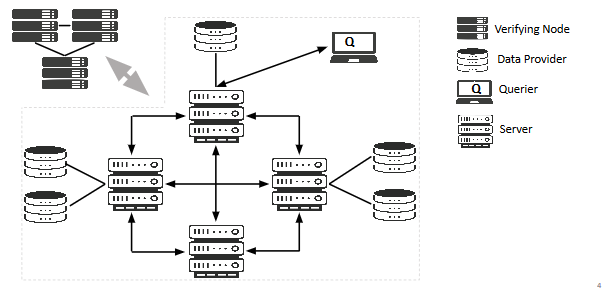
\includegraphics[scale=0.75]{img/lemal.png}
\caption{System model of Lemal}
\end{figure}
Lemal is a privacy-preserving data sharing system developed in collaboration of this project by LCA1. It consists of a collective authority (CAà formed by $m$ servers, $S_1,...S_m$ and $n$ data providers $DP_1,...DP_n$ containing sensitive data, encrypted using EC ElGamal.
Another collective authority of verifying nodes is linked to this system, which maintains the distributed ledger, is described in Section 5. This sytem is used to answer queries made by a querier $Q$, to produce results of some aggregate functions. Each DPs choose one server of the CA to communicate with and can change this at any given time.\\
\textbf{Functionality}: Lemal permits a large set of SQL queries, like \textit{Where, group by, like, mean, variance, set intersection}, with some machine learning (\textit{linear and logistic regression}) and Private recommender system functionality such as \textit{cosine similarity, CBF-Based recommendations, ...}.\\
For any query, proofs are computed and stored by verifying nodes in a skipchain so that any party can verify what has been done.
\subsection{Threat Model}
\begin{figure}[H]
\center
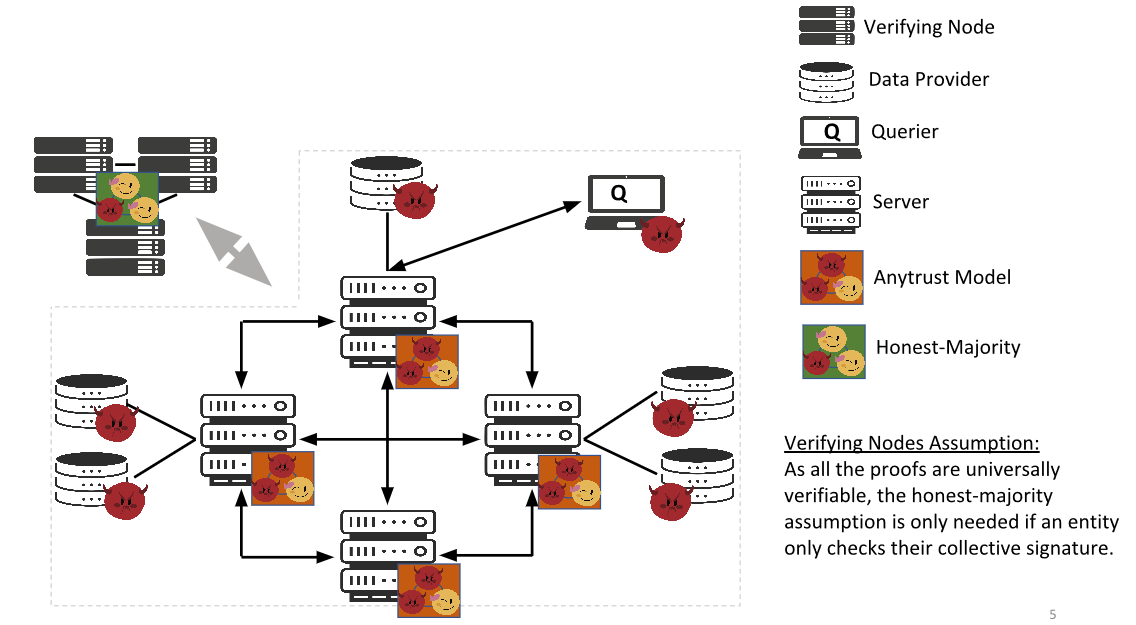
\includegraphics[scale=0.75]{img/threatLemal.png}
\caption{Threat model of Lemal}
\end{figure}
\textbf{Collective authority servers} It is assumed an Anytrust model [14]. It does not require a particular server to be trusted or to be honest-but-curious. Whenever one of the server is not malicious, functionnality, security and privacy are guaranteed.\\
\textbf{Collective authority verifying nodes} It is assume an Hones majority. Meaning a threshold of more than half of the nodes are honest, and the consensus is done via Byzantine fault tolerance protocol.\\
\textbf{The Querier, and Data providers} are assumed malicious. They can collude between themselves or with a subset of the CA servers.\\
It is also assumed that all network communication is encrypted and authenticated by using a protocol such as TLS or SSL.
\subsection{Properties}
\textbf{Confidentiality} All data are encrypted using EC ElGamal, no party sees the data in clear, except the Querier that get the aggregate result encrypted under his public key. This property holds as long as one server is honest
\textbf{Privacy} First, one step of the protocol of Lemal is shuffling, that ensures \textbf{unlinkability} between DPs and their data. Then, it ensure \textbf{differential privacy} for any individual sharing its data.\\
In any case, privacy of the querier is not adressed in this system, but only the sensitive data of the DPs.
\textbf{Correctness} At each step of the protocol, zero-knowledge, non interactive proofs are generated by the CA server. These proofs can be used between two steps to verify that computation were correctly done, and if its not it can identified the entity that did not compute correctly.
\textbf{Robustness}

\subsection{Query example}
This subsection details the pipeline of a query process.\\
First, the querier $Q$ send a query to the CA server. The example taken in this section is "SELECT average(x) FROM y WHERE y.z = 3".\\
This query is received by a server $s$ of the CA, and broadcasted to the entire CA. Then each server sends to its DPs, the query. The DPs execute it locally, then send the result encrypted with the CA's public key to each server that send them the query.\\
At this point each server of the CA contains ciphers encrypted with the CA's public key. A shuffling phase is initiated

\section{Verifying Node}
\subsection{System Model}
\subsection{Threat Model}
\subsection{Type of Proofs}
\subsection{Operation supported}

\section{Implementation}

\section{Performance Evaluation}
\section{Conclusion and Future Work}
\begin{thebibliography}{9}
\bibitem{prioimple}
Henry Corrigan-Gibbs, Prio prototype implementation\\
\texttt{https://github.com/henrycg/prio}
\end{thebibliography}
\end{document}
